\documentclass[12pt]{article}
\usepackage{amsmath,amsfonts,amssymb}
\usepackage{graphicx}
\usepackage{hyperref}
\usepackage{authblk}

\title{Observer-Centric Bitstring Universes: A Minimal Informational Model of Reality}
\author{Juha Meskanen}
\date{July 2025}

\begin{document}

\maketitle

\begin{abstract}
    We present a discrete, observer-based model of the universe grounded in bitstring information theory. In this minimal setting, we define observers as sequences of finite bitstrings and investigate their persistence within possible universes composed of frames of bits. The model introduces a similarity metric for observer survival, proposes an entanglement-like phenomenon via shared memory fragments, and reinterprets the wavefunction as a compressed extrapolation over observer trajectories. This framework challenges traditional physical ontology, suggesting that reality is observer-centric and informational at its core.
\end{abstract}

\section{Introduction}

We explore a radically minimalist foundation for physics, based on bitstrings and observer-centric reasoning. In this model, the universe is not something that evolves over time from a dynamical rule, but rather a collection of static information patterns in which observers may find themselves embedded. Observers persist through time only by re-identifying themselves across similar structures. Thus, what we call \emph{reality} is the subset of bitstring universes that contain coherent observer trajectories.

\section{Framework and Definitions}

Let $B$ be the number of total bits used to describe a universe. We define:

\begin{itemize}
    \item $\mathcal{U}_B$: the set of all possible universes composed of bitstrings of length $B$, partitioned into frames $f_i$ representing temporal slices.
    \item $O = \{o_1, o_2, \ldots, o_n\}$: a sequence of bitstrings representing the observer's memory and state across subjective time.
\end{itemize}

\subsection{Observer-Centric Universe Construction Principle (OCUCP)}

An observer is said to exist only in those universes $U \in \mathcal{U}_B$ such that for all $i$, there exists $o_i \subseteq f_i$. That is, the observer must be embedded, frame by frame, into the universe.

This approach inverts the usual ontology: rather than universes determining observers, observers determine which universes are relevant. Reality is defined \emph{relative to the observer's compatibility with the universe}.

\subsection{Observer Memory Lemma (OML)}

Let $O = \{o_1, o_2, \ldots, o_n\}$ be an observer trajectory, and $F = \{f_1, f_2, \ldots, f_n\}$ be a candidate sequence of universe frames. Then, the observer can only \emph{remember} or \emph{experience} $F$ if:

\[
    \exists\ \epsilon > 0\ \text{ such that }\ \text{Similarity}(o_i, f_i) \ge \epsilon\ \text{ for all } i.
\]

That is, the observer's internal structure must have sufficient overlap with the universe frames in order for continuity and memory to be possible. Memory is structural self-similarity over time, not causal flow.

\subsection{Similarity Metric and Observer Survival}

We define a similarity function $\text{Sim}(a, b)$ between two bitstrings. An observer $O$ survives across a frame transition $o_i \to o_{i+1}$ only if $\text{Sim}(o_i, o_{i+1}) \ge \delta$ for some threshold $\delta$. This defines a selection criterion over trajectories.

\section{Compression and the Wavefunction}

We propose a new interpretation of the quantum wavefunction, grounded in the logic of observer survival under compression.

\subsection{Compression Bias Principle (CBP)}

Let $C(F)$ be the compressed length of universe frames $F = \{f_1, \ldots, f_n\}$. Then the number of observers that can embed within $F$ is inversely correlated with $C(F)$.

That is, smooth, regular, and compressible universes support more observers, simply because more observer trajectories can fit into the same limited bit budget. Hence, the universe we find ourselves in is likely to be highly compressible.

\subsection{Wavefunction as Compressed Continuation}

An observer predicts future frames by extrapolating structural regularities from their memory using compression logic:

\begin{itemize}
    \item The observer contains past states $\{o_1, \ldots, o_t\}$.
    \item They extrapolate possible futures $o_{t+1}, \ldots, o_{t+k}$ using pattern completion.
    \item If the compression basis is Fourier/sine-based (e.g., JPEG), this extrapolation leads to smooth predictions.
    \item Multiple continuations are possible, forming a "superposition" in the observer's internal model.
\end{itemize}

Interference arises when extrapolated continuations reuse shared substrings. Thus, quantum phenomena emerge not from physical superposition, but from ambiguous extrapolations under compression logic. This model views the wavefunction as an efficient coding scheme, not a physical object.

\section{Entanglement and Shared Memory}

Entanglement is modeled as mutual constraint between observer subcomponents. If two observer bitstrings $A$ and $B$ share internal fragments and exist within a common universe $U$, then the observer can only survive in frames that preserve both. This shared structure constrains joint probabilities, simulating entanglement.

This is a structural, non-local correlation — not a causal interaction. It arises because the observer is one unified bitstring with branching substructures, not two separate agents.


\section{Simulation Output Samples}

Here we provide sample outputs from the Python simulation constructing universes of fixed bit length,
evaluating observer embedding and survival scores over time.


\begin{figure}[h!]
    \centering
    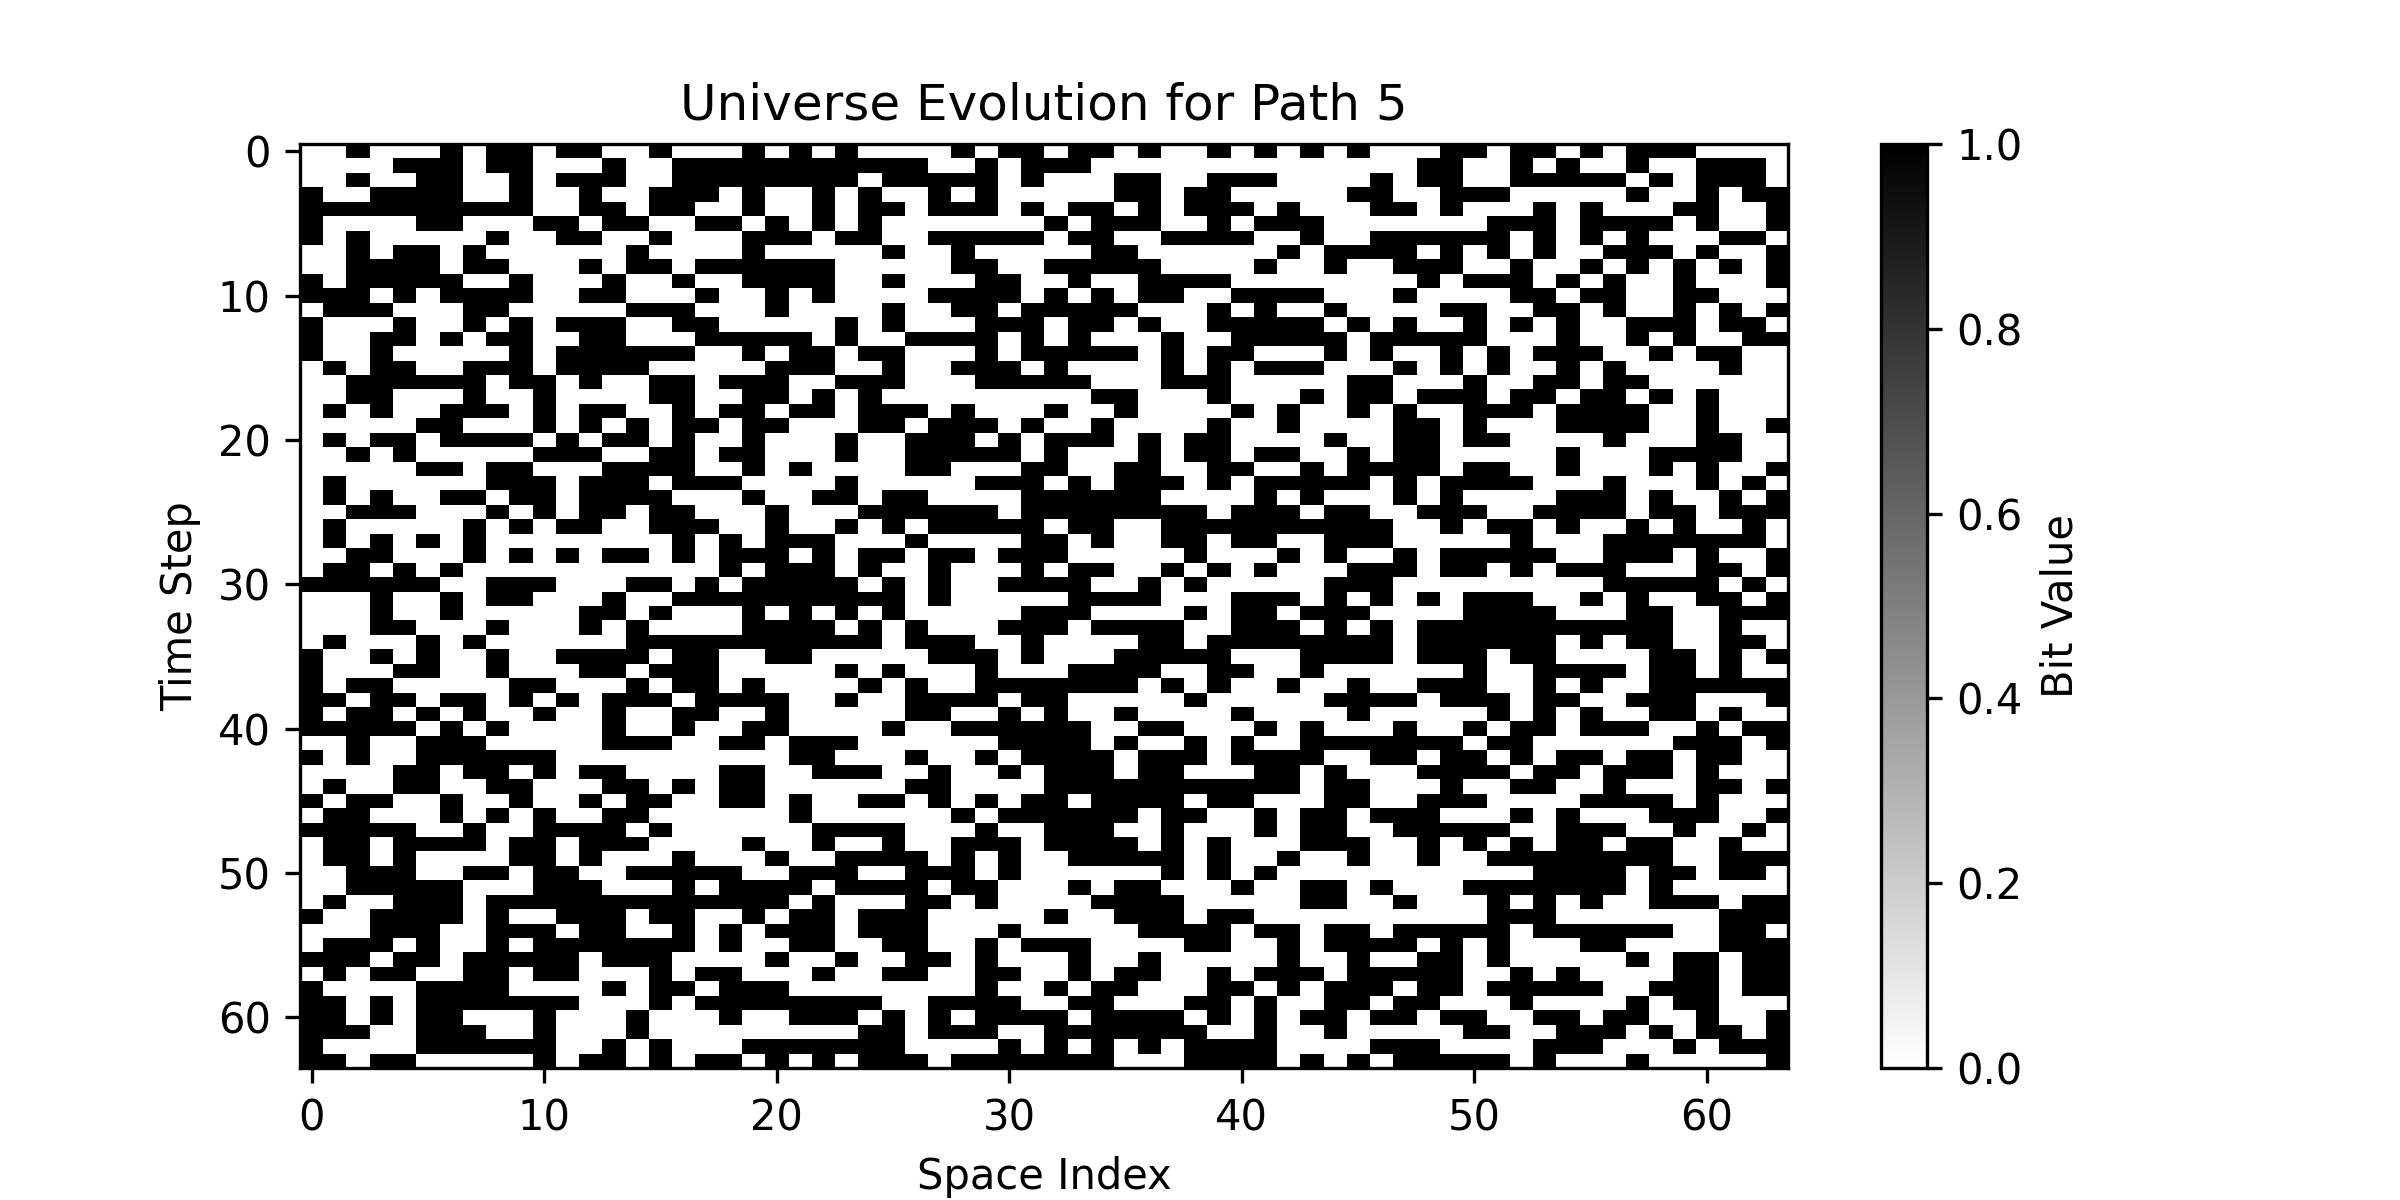
\includegraphics[width=1.0\textwidth]{figures/state_evolution_heatmap.png}
    \caption{State evolution of one possible universe defined by a bitstring of 12 bits, with observer included. The evolution
        demonstrate coherence}
    \label{fig:state_evolution}
\end{figure}

\begin{figure}[h!]
    \centering
    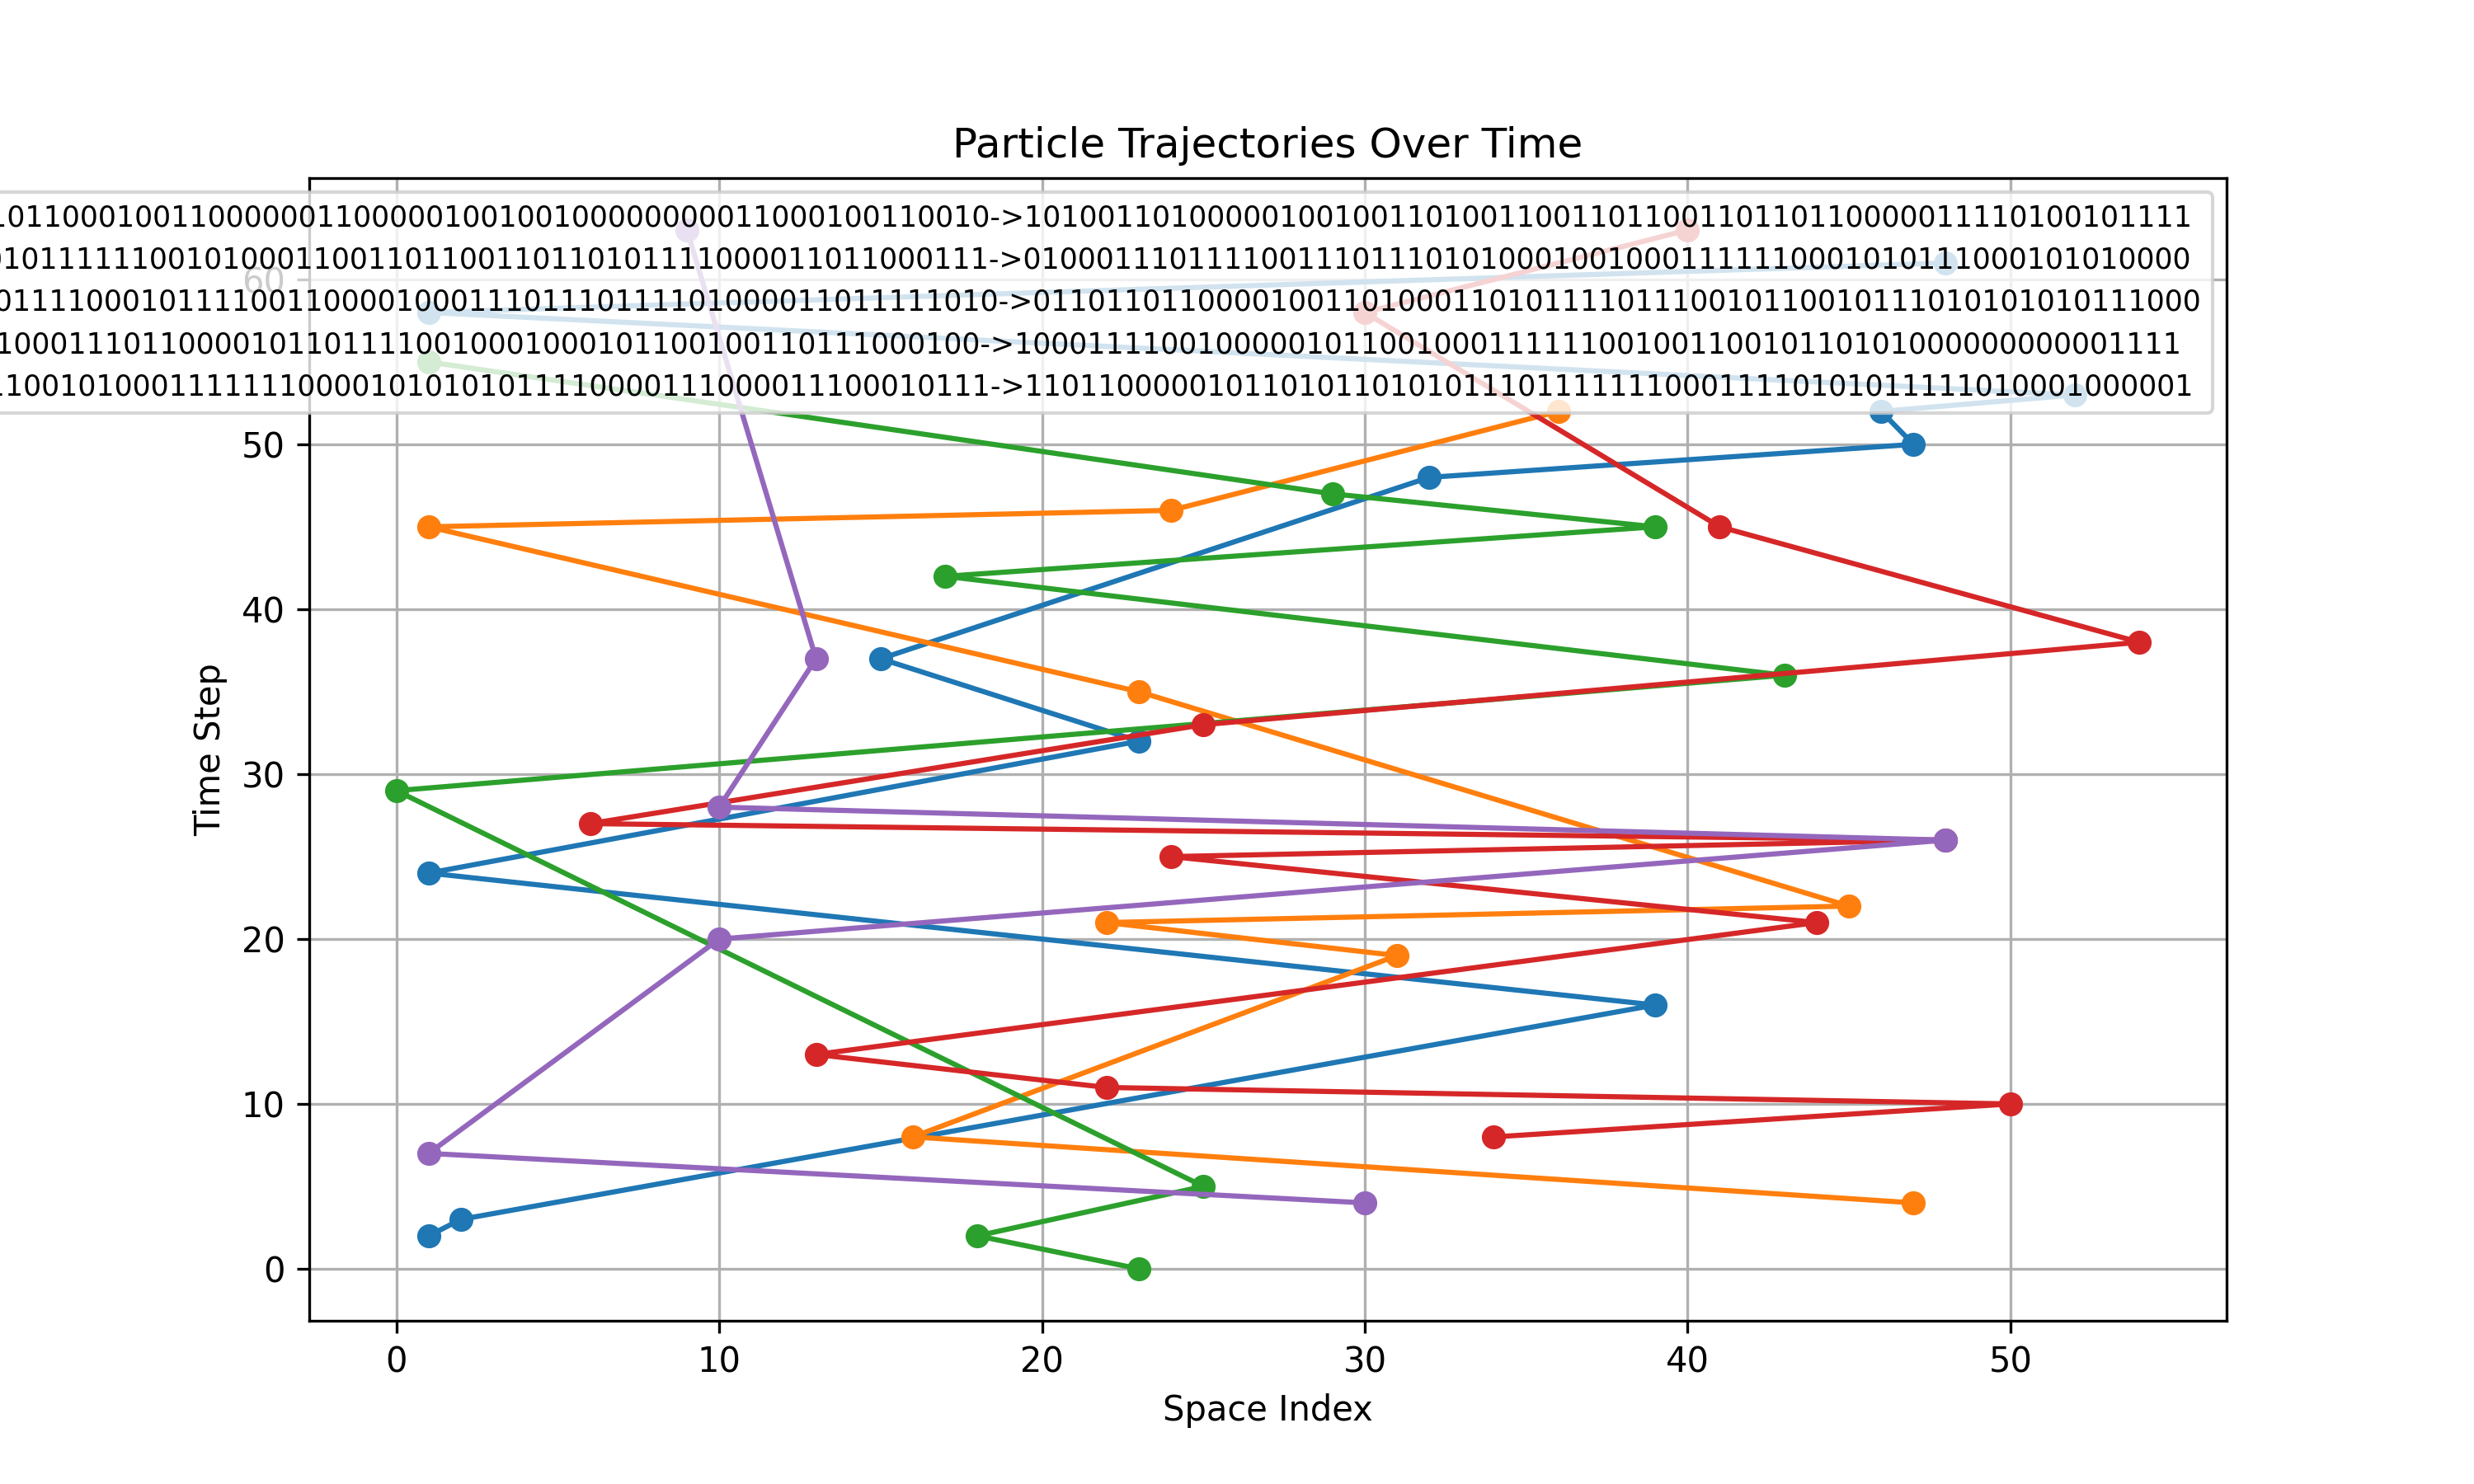
\includegraphics[width=1.0\textwidth]{figures/particle_trajectories.png}
    \caption{Particle traces demonstrating smooth trajectories emerge in worlds that include observer pattern}
    \label{fig:particle_trajectories}
\end{figure}



\section{Discussion and Implications}

This model abandons conventional notions of causality and dynamics in favor of a static informational ontology. Universes do not evolve; rather, they are sampled by the observer based on compatibility. The past is defined by fragments present in memory; the future is an extrapolation constrained by compression logic.

There is no fundamental substrate — only bitstrings and the observer's search for consistent continuations. Gravity, time, and quantum effects emerge as statistical preferences under this framework.

\section{Conclusion}

We proposed a minimal observer-centric framework in which the universe is composed of bitstrings, and persistence is governed by similarity and compression. Observer memory is realized through structural overlap, and probability emerges from counting consistent embeddings. This framework provides a possible foundation for reconciling quantum and classical views under informational realism.

\end{document}

